\section{Pianificazione}
	In seguito alla suddivisione delle scadenze, per eseguire una più accurata pianificazione progettuale, il progetto è stato suddiviso nei seguenti periodi: \\
	\begin{itemize}
		\item \textbf{Analisi};
		\item \textbf{Consolidamento dei requisiti};
		\item \textbf{Progettazione Architetturale};
		\item \textbf{Progettazione di Dettaglio e Codifica};
		\item \textbf{Verifica e Validazione}. \\
	\end{itemize}
	Ognuno di questi periodi è stato poi suddiviso in più attività, a ognuna delle quali sono state associate una o più risorse. Ogni attività è stata suddivisa in sotto-attività, delle quali sono stati riportati i Diagrammi di \glossaryItem{Gantt} così da evidenziare la pianificazione di dettaglio restando focalizzati sui concetti di maggiore importanza.
	\subsection{Analisi}
	\textbf{Periodo:} da 2017-02-23 a 2017-04-03 \\
	Questa fase inizia in concomitanza con la pubblicazione dei capitolati d'appalto e termina in 		 corrispondenza della \textbf{Revisione dei Requisiti}. \\
	Le attività principali del periodo di \textbf{Analisi} sono: \\
	\begin{itemize}
		\item \textbf{Norme di Progetto:} L'\textit{Amministratore}, sottoscrive tutte le regole che il gruppo è obbligatoriamente tenuto a seguire durante l'attuazione di tutte le attività progettuali. In questo documento devono quindi essere inserite tutte le norme e le scelte del software di supporto non vincolate al capitolato. Sarò poi compito dei verificatori la certificazione del rispetto di tali norme;
		\item \textbf{Studio di Fattibilità:} Vengono discussi e valutati dal gruppo tutti i capitolati d'appalto. Viene quindi redatto il documento \textbf{Studio di Fattibilità}, contenente i risultati di tali analisi. L'attività di analisi consiste nel valutare della complessità delle varie proposte mediante l'abbozzo di \textit{Analisi dei Requisiti} ad alto livello. La stesura di questo documento è necessaria per la creazione degli altri documenti in quanto è proprio da questo documento che emerge il progetto che il gruppo porterà avanti;
		\item \textbf{Analisi dei Requisiti:} Partendo dalla bozza di \textit{Analisi dei Requisiti} redatta durante lo \textit{Studio di Fattibilità}, si esegue un analisi più approfondita. Tale attività continuerà fino alla data di consegna stabilita;
		\item \textbf{Piano di Progetto:} Il \textit{Responsabile di Progetto}, basandosi sulle date di scadenza, redige il documento Piano di Progetto, organizzando tutte le attività del gruppo per lo svolgimento del lavoro. Tale attività ha una priorità alta in quanto regola le attività svolte dall'intero gruppo;
		\item \textbf{Piano di qualifica:} Si individuano tutte le strategie di verifica e validazione che il gruppo dovrà adottare per il progetto. La documentazione del \textit{Piano di Qualifica} viene redatta da un \textit{Analista} in collaborazione con l'\textit{Amministratore} ed il \textit{Responsabile di Progetto};
		\item \textbf{Glossario:} I redattori, parallelamente alla stesura degli altri documenti, creano un documento che contiene una selezione di termini usati nella stesura della documentazione che necessitano di disambiguazione. Per ognuno di questi vocaboli presenti nel Glossario si associa una definizione al fine di chiarire il significato del termine all'interno del progetto. Il documento viene quindi aggiornato in maniera incrementale ad ogni inserimento di un nuovo termine;
		\item \textbf{Lettera di presentazione:} Viene redatta una lettera da presentare al Committente per permettere al gruppo di partecipare alla gara d'appalto per il capitolato. \\
	\end{itemize}
	\subsubsection{Diagramma di Gantt delle attività}
	\begin{figure}[H]
		\centering
		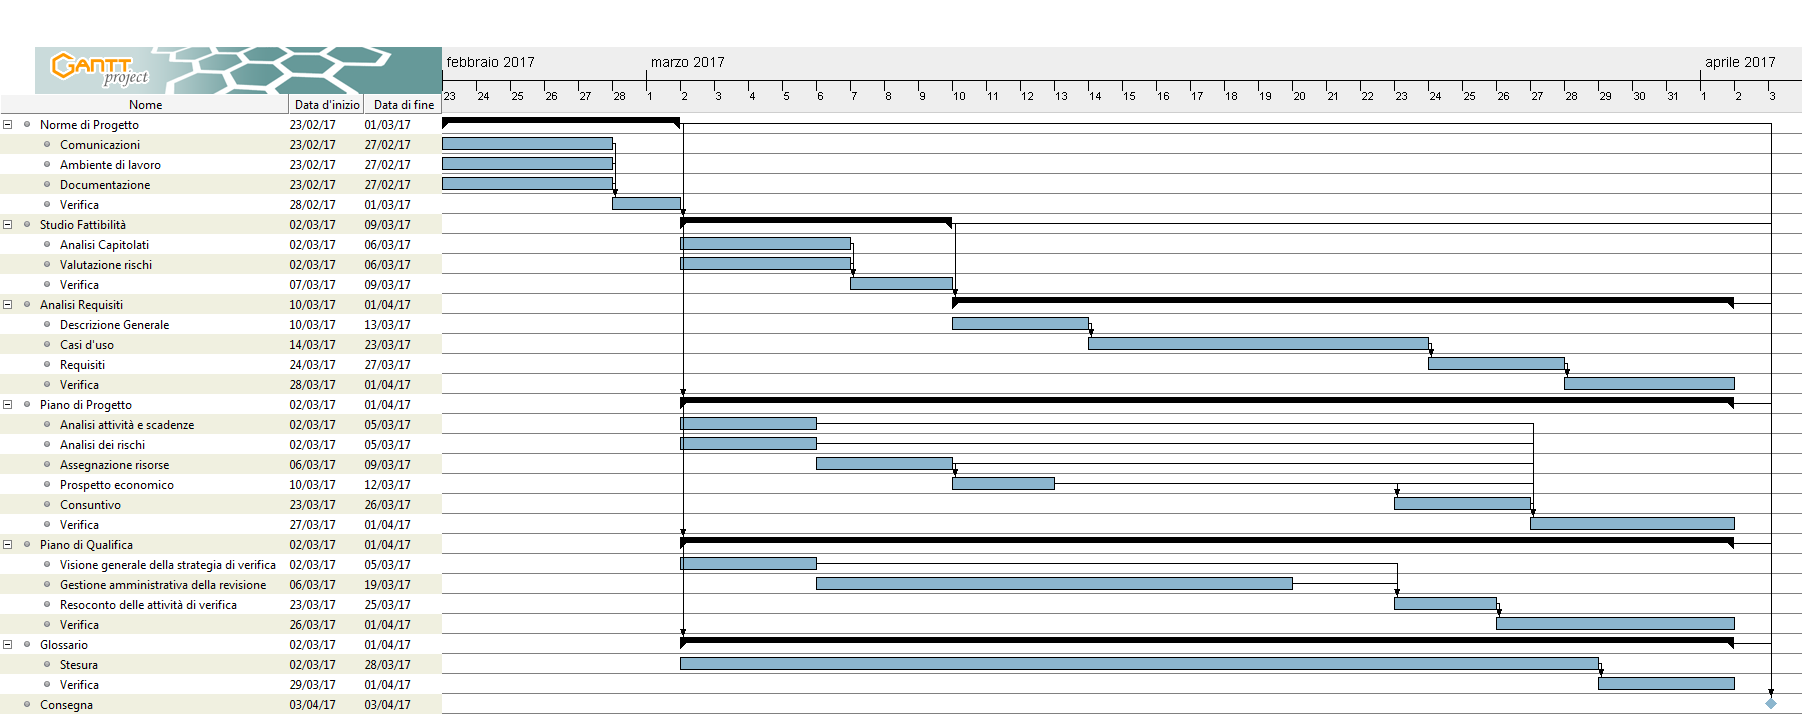
\includegraphics[width=1\linewidth]{immagini/gantt/analisi.png}
		\caption{Diagramma di Gantt, periodo di Analisi}
	\end{figure}
	\subsection{Consolidamento dei Requisiti}
	\textbf{Periodo:} da 2017-04-10 a 2017-04-18 \\
	Questo periodo inizia successivamente alla \textbf{Revisione dei Requisiti} e si conclude con l'inizio del periodo di \textbf{Progettazione Architetturale}. \\
	Vengono consolidati i requisiti richiesti dal sistema e per viene migliorato il documento \textit{Analisi dei Requisiti}. \\
	\subsubsection{Diagramma di Gantt delle attività}
	\begin{figure}[H]
		\centering
		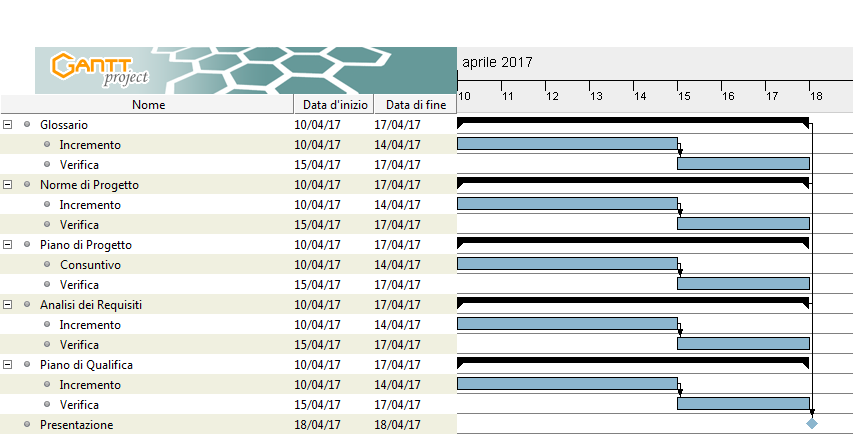
\includegraphics[width=1\linewidth]{immagini/gantt/consolidamento_requisiti.png}
		\caption{Diagramma di Gantt, periodo di Consolidamento dei Requisiti}
	\end{figure}
	\subsection{Progettazione Architetturale}
	\textbf{Periodo:} da 2017-04-19 a 2017-05-15 \\
	Questo periodo inizia al termine del \textbf{Consolidamento dei Requisiti} e termina con la consegna del prodotto alla \textbf{Revisione di Progettazione} minima. \\
	Le attività principali del periodo di \textbf{Progettazione Architetturale} sono: \\
	\begin{itemize}
		\item \textbf{Specifica Tecnica:} Il \textit{Responsabile di Progetto} descrive al gruppo le scelte progettuali, ad alto livello, che il prodotto dovrà rispettare. Inoltre, vengono esposti i \glossaryItem{Design Pattern} che verranno utilizzati nella creazione del prodotto, l'architettura generale del software, i principali flussi di controllo e il tracciamento dei requisiti;
		\item \textbf{Incremento e verifica:} Tutti i documenti verranno aggiornati in base al risultato
della \textit{Revisione dei Requisiti}. \\
	\end{itemize}
	\subsubsection{Diagramma di Gantt delle attività}
	\begin{figure}[H]
		\centering
		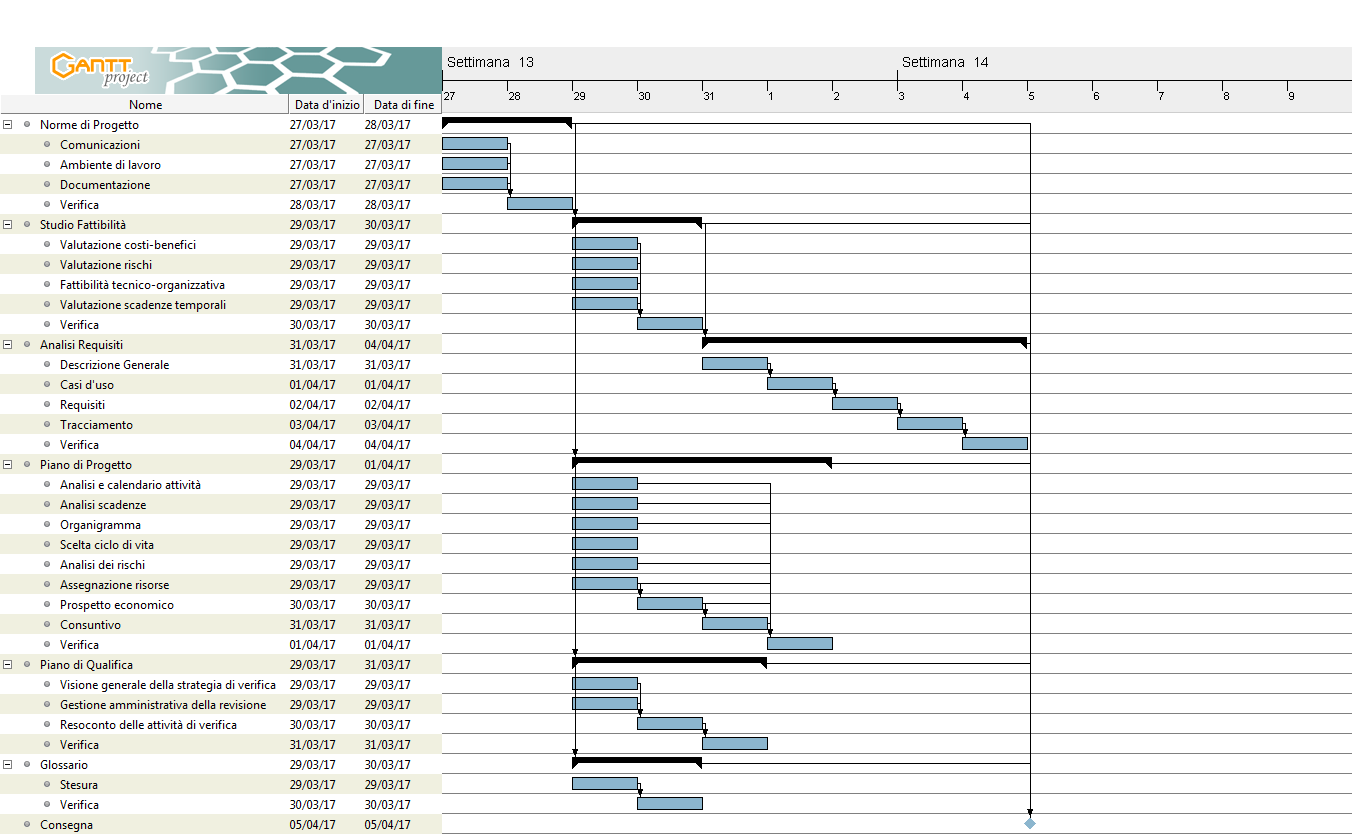
\includegraphics[width=1\linewidth]{immagini/gantt/progettazione_architetturale.png}
		\caption{Diagramma di Gantt, periodo di Progettazione Architetturale}
	\end{figure}
	\subsection{Progettazione di Dettaglio e Codifica}
	\textbf{Periodo:} da 2017-05-16 a 2017-07-13 \\
	Questo periodo inizia dopo la \textbf{Revisione di Progettazione} e termina con la consegna del prodotto alla \textbf{Revisione di Qualifica}. Le attività principali del periodo di \textbf{Progettazione di Dettaglio e Codifica} sono: \\
	\begin{itemize}
		\item \textbf{Definizione di Prodotto:} Viene redatto il documento \textit{Definizione di Prodotto}. All'interno di tale documento vengono definite approfonditamente la struttura e le relazioni dei vari componenti del prodotto, basandosi sul documento \textit{Specifica Tecnica};
		\item \textbf{Codifica:} Si procede allo sviluppo del codice del software da parte dei programmatori, seguendo quanto è riportato nella \textit{Definizione di Prodotto};
		\item \textbf{Manuali utenti:} Si creano i documenti che hanno lo scopo di fornire delle linee guida per l'utilizzo del sistema da parte degli utenti coinvolti;
		\item \textbf{Incremento e verifica:} Si devono aggiornare tutti i documenti basandosi sui risultati della \textbf{Revisione di Progettazione}. \\
	\end{itemize}
	\subsubsection{Diagramma di Gantt delle attività}
	\begin{figure}[H]
		\centering
		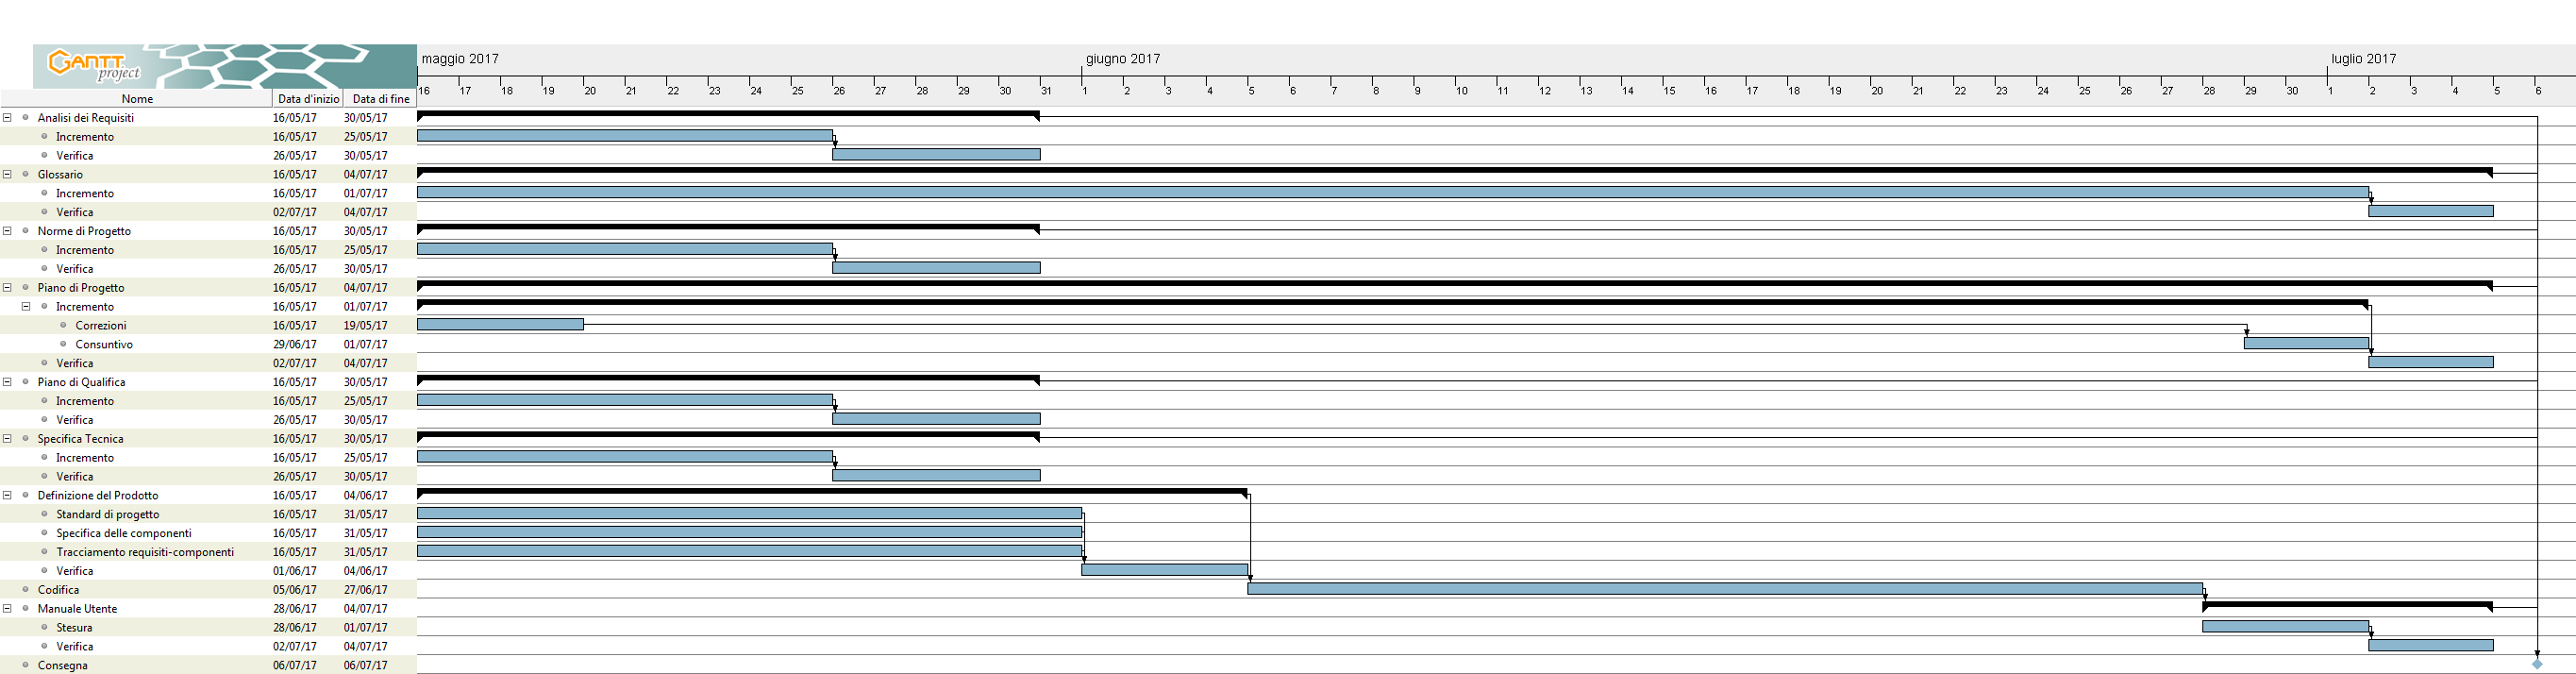
\includegraphics[width=1\linewidth]{immagini/gantt/progettazione_dettaglio_codifica.png}
		\caption{Diagramma di Gantt, periodo di Progettazione di Dettaglio e Codifica}
	\end{figure}
	\subsection{Verifica e Validazione}
	\textbf{Periodo:} da 2017-07-14 a 2017-08-29 \\
	Questo periodo inizia dopo la \textbf{Revisione di Qualifica} e termina il processo di sviluppo del software. Tale fase rappresenta l'atto conclusivo delle varie attività di verifica realizzate nei singoli processi del Ciclo di vita. \\
	Le attività principali del periodo di \textbf{Verifica e Validazione} sono: \\
	\begin{itemize}
		\item \textbf{Collaudo del sistema:} in questa attività il prodotto viene collaudato per dare
dimostrazione che è conforme alle specifiche e soddisfa tutti i requisiti stabiliti;
		\item \textbf{Incremento e verifica:} in questa attività tutti i documenti vengono aggiornati in base al risultato della \textbf{Revisione di Qualifica}. \\
	\end{itemize}
	\subsubsection{Diagramma di Gantt delle attività}
	\begin{figure}[H]
		\centering
		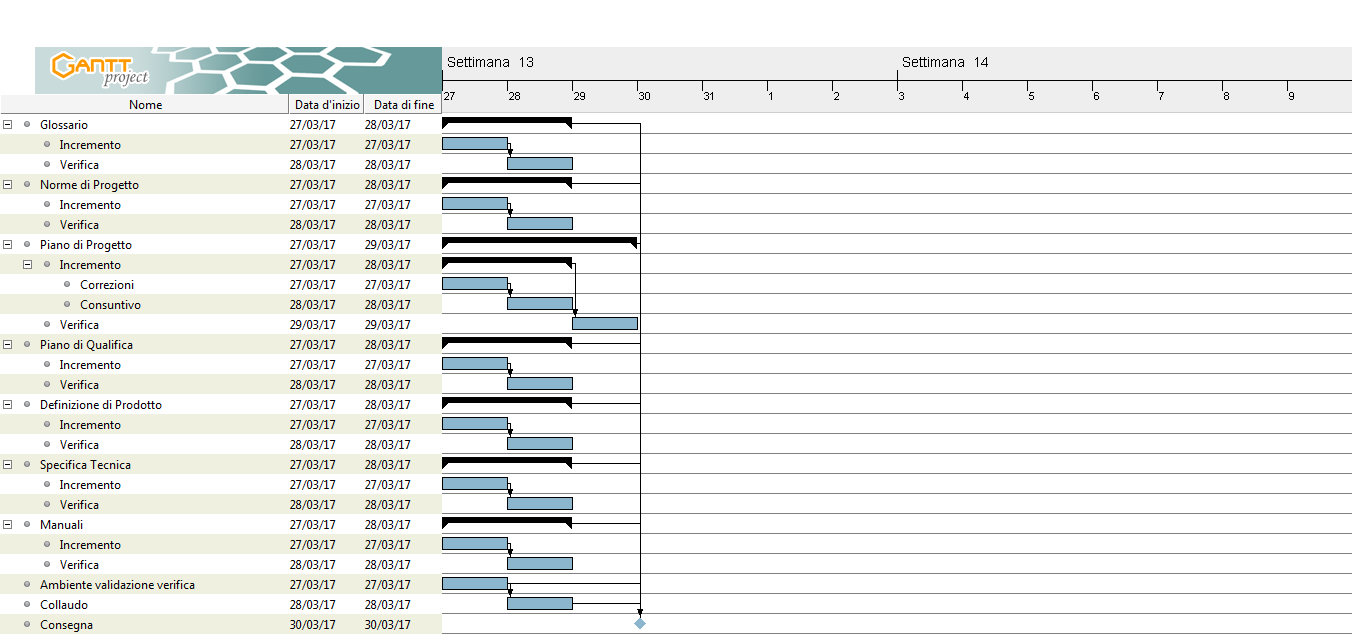
\includegraphics[width=1\linewidth]{immagini/gantt/validazione.png}
		\caption{Diagramma di Gantt, periodo di Verifica e Validazione}
	\end{figure}